\section{Approach Overview}
\label{sec:appro}

In this section, we describe the general framework of our system
to extract the structured textual information from the medical images.
A running example will be given to detail the different parts of the system.

\subsection{Framework}
\begin{figure*}[ht]
%\begin{figure}[H]
\centering
\epsfig{file=figure/framework.eps, width=1.8\columnwidth}
\caption{System Framework}
\label{fig:framework}
\end{figure*}

% here's the Framework
\figref{fig:framework} shows the framework of the whole system.
% image: same formats
The system takes as input one or more medical images of the same format
(e.g., the same medical test conducted by the same equipment).
All images are processed by the OCR engine,
turning into raw OCR results in a structured format such as XML.
For each raw OCR result,
we ignore its hierarchy and collect all the leaf text boxes as the OCR data,
denoted by $D$.
As defined in \equref{equ:data}, each leaf text box $d$ is a 5-tuple,
which contains the left, top, right, bottom coordinates
with the recognized text respectively.
\begin{equation}
  D = \{d_1, ..., d_n\}, \quad d = (x_0, y_0, x_1, y_1, text).
\label{equ:data}
\end{equation}

% ODL: annotated by user through a simple graphical user interface.
The other part of the input is the data description of those images,
written in ODL.
In a practical system, a user can annotate the data description through
a graphical user interface, which allows defining strings and variables,
adding data constraints and drawing \textit{rough} bounding boxes for different
elements in the image.
Afterwards, the corresponding ODL description is automatically generated.

% Given ODL, parser begin to work, returning one parsing tree.
The parsing process is the main part of our system.
Given the OCR data $D$ and user-defined ODL, we propose the ODL parser
which matches all the elements in the provided description
with the text from $D$, and produces parsing results.
The parsing results are in the form of a parsing tree, where every leaf node
contains both the element of ODL and the corresponding text information.
% what's fuzzy
% The word ``fuzzy'' means that the parser
The parser tolerates the errors of OCR recognition and slight layout variances
during the extracting process,
therefore it's able to produce multiple candidate parsing trees
with slight mismatches,
and the most suitable result will be selected using scoring functions.
% TODO: What's parsing tree, shall I put the formal definition here?
% TODO: What's the suitable formal definition?

% Finally: correction model.
In addition, the system contains an automatic correction module,
which learns OCR recognition errors and tries to correct errors
during the parsing phase.
After parsing multiple images, the system collects all detected parsing errors,
then provide the user with most frequent parsing errors and
prompt the user for possible corrections.
Such corrections would then be incorporated into a correction model,
which guides the parser to make possible corrections
during the subsequent parsing process, and results in fewer errors.

% In next few subsections, we will present a running example, using
% an ECG image, with
% which we will explain the syntax and semantics of ODL,
% as well as the interactive human correction mechanism in this framework.
% The techniques developed in this section can be applied to
% other types of semi-structured medical images as well.

%The main components of our system are as follows:
%\begin{enumerate}
%\item The OCR engine generates XML files which contain both the recoginized text and the corresponding coordinates information.
%\item The fuzzy parser, which is automatically generated based on the image description, is used to parse the XML files and extract the information.
%\item The fuzzy parser will suggest some errors for human to correct, after that the correction model which is used for fuzzy parsing will be updated based on the correction that human made.
%\end{enumerate}

\subsection{Running Example}
We continue using the ECG in \figref{fig:running-ecg} as the running example.
We are interested in extracting the time, measurements and some basic diagnoses,
all highlighted in the red ovals.
Fragments of the XML results produced by the OCR software are shown in \figref{fig:running-xml}.
% In addition, spatial coordinates for different
% OCR units, like paragraphs, lines and words, are recorded as values
% for the ``title'' attribute in XML.

% \begin{figure}[ht]
% \centering
% \subfigure[]{
% \label{fig:subfig:a}
% \begin{minipage}[b]{0.2\textwidth}
\newsavebox{\thirdlisting}
\begin{lrbox}{\thirdlisting}% Store first listing
\small
\begin{lstlisting}[basicstyle=\tiny,]
*$union$* month_str{
    "Jan"; "Feb"; "Mar";
    "Apr"; "May"; "Jun";
    "Jul"; "Aug"; "Sept";
    "Oct"; "Nov"; "Dec";
};
*$union$* month_t{
    *$int$*(1,12)  num;
    month_str str;
};
*$struct$* time_t{
    *$int$*(1,31)  day;
    "-";
    month_t month;
    "-";
    *$int$*()    year;
};
*$struct$* triple_t{
    "Vent. rate";
    *$hskip$*(\t)  skip;
    *$int$*(60,100)  vr;
    "bpm";
};
\end{lstlisting}
\end{lrbox}
% \end{minipage}
% }
% \hspace[1in]
% \subfigure[]{
% % \label{fig:subfig:b}
% % \begin{minipage}[b]{0.2\textwidth}
\newsavebox{\forthlisting}
\begin{lrbox}{\forthlisting}
\begin{lstlisting}[basicstyle=\tiny,]
*$union$* interpretation_t{
    "Normal ECG";
    "Abnormal ECG";
};
*$struct$* parameter_t{
    *$int$*()  p1;
    "Hz";
    *$float$*(3, 1)    p2;
    "mm/s";
    *$float$*(3, 1)    p3;
    "mm/mV";
};
*$source$* *$struct$* entry_t{
    time_t(<0.0w,0.0h,1.0w,0.3h>)  time;
    triple_t(<0.1w,0.0h,0.5w,1.0h>)  tri;
    interpretation_t(<0.3w,0.0h,1.0w,0.5h>)  inter;
    *$vskip$*(\n)[]  skipline;
    parameter_t  para;
};
\end{lstlisting}
\end{lrbox}
% % \end{minipage}
% }

\begin{figure*}[ht]
\centering
\subfloat{
% \label{fig:description:a}
\scalebox{1.6}{\usebox{\thirdlisting}}
}
\hspace{1.5cm}
\subfloat{
% % \label{fig:description:b}
\scalebox{1.6}{\usebox{\forthlisting}}
}
\caption{The ODL description in surface syntax.}
\label{fig:running-odl-surface}
\end{figure*}

% \lipsum[2]


There are numerous ways to describe the image using ODL.
One of the descriptions is shown in \figref{fig:running-odl-surface},
written in the surface syntax.
In the description,
% basic: fixed strings, or variables (year, date, bpm)
the simplest expressions are fixed constants and primitive variables.
For example, \textit{``Vent. rate''} is a string constant,
and \textit{num} is the name of an integer variable ranging from 1 to 12.
Users can customize compound types
for representing structured textual information.
For instance, \textit{time\_t} is a \textit{struct} type representing
day, month and year information;
\textit{month\_str} is a \textit{union} type representing enumerable month abbreviations.
% root: source
Users can further specify rough bounding boxes for different expressions.
As what depicted in the description,
the variable \textit{time} has a rough zone, indicating
the corresponding data resides in the top 30\% area of the whole image.
The keyword \textit{source} stands for the root expression
of the entire data to be extracted.
In addition, the corresponding abstract syntax of this description is shown in \figref{fig:running-odl-abstract},
and our later discussion on ODL will use the \textbf{abstract syntax} as instead.

% \begin{figure}[ht]
% \centering
% \subfigure[]{
% \label{fig:subfig:a}
% \begin{minipage}[b]{0.2\textwidth}
\newsavebox{\absflisting}
\begin{lrbox}{\absflisting}% Store first listing
\begin{lstlisting}[basicstyle=\tiny,]
    {

        {
            day(int, 1, 31),
            "-",
            {
                num(int, 1, 12) |
                {
                    "Jan" | "Feb" | "Mar" | 
                    "Apr" | "May" | "Jun" | 
                    "Jul" | "Aug" | "Sept" | 
                    "Oct" | "Nov" | "Dec"
                }
            }
            "-",
            year(int)
        }(<_,_,_,0.3l>),

        {
            "Vent. rate",
            *$hskip$* \s,
            x(int, 60, 100),
            "bpm",
        }(<0.1w,_,0.5w,_>) as triple,

        {
            "Normal ECG" | 
            "Abnormal ECG"
        }(<triple.x1,triple.y0,_,_>),

        *$vskip$* \n list
        
        {
            p1(int),
            "Hz",
            p2(float, 3, 1),
            "mm/s",
            p3(float, 3, 1),
            "mm/mV"
        }(<_,_,_,_>)
    }
\end{lstlisting}
\end{lrbox}

% \newsavebox{\absflisting}
% \begin{lrbox}{\absflisting}% Store first listing
% % \fontsize{6pt}{7pt}\selectfont
% \begin{lstlisting}
%     {

%         {
%             day(int, 1, 31),
%             "-",
%             {
%                 num(int, 1, 12) |
%                 {
%                     "Jan" | "Feb" | 
%                     "Mar" | "Apr" |
%                     "May" | "Jun" | 
%                     "Jul" | "Aug" |
%                     "Sept" | "Oct" | 
%                     "Nov" | "Dec"
%                 }
%             }
%             "-",
%             year(int)
%         }(<_,_,_,0.3l>),

%         {
%             "Vent. rate",
%             *$hskip$* \s,
%             x(int, 60, 100),
%             "bpm",
%         }(<0.1w,_,0.5w,_>) as triple,
% \end{lstlisting}
% \end{lrbox}


% \newsavebox{\absslisting}
% \begin{lrbox}{\absslisting}
% % \fontsize{6pt}{7pt}\selectfont
% \begin{lstlisting}
%         {
%             "Normal ECG" | 
%             "Abnormal ECG"
%         }(<triple.x1,triple.y0,_,_>),

%         *$vskip$* \n list
        
%         {
%             p1(int),
%             "Hz",
%             p2(float, 3, 1),
%             "mm/s",
%             p3(float, 3, 1),
%             "mm/mV"
%         }(<_,_,_,_>)
%     }
% \end{lstlisting}
% \end{lrbox}
% % \end{minipage}

\begin{figure}[!ht]
\centering
\small
% \subfloat
% \label{fig:absdes:a}
\scalebox{1}
{\usebox\absflisting}
% \hfill
% \subfloat
% % \label{fig:absdes:b}
% {\usebox\absslisting}
\caption{ODL Description in Abstract Syntax}
\label{fig:absdes}
\end{figure}

% \lipsum[2]


The example parsing tree is shown in \figref{fig:running-parsing-tree},
where leaf nodes are either (constant, value) or (variable, value) pairs.
The node \textit{entry\_t} serves as the root node of the whole tree,
and leaf nodes are marked with ``Error'' if an imperfect alignment is detected,
either because the constant and value doesn't exactly match,
or because the value doesn't satisfy the corresponding value constraint.
The system will prompt frequent parsing errors for manual corrections.
For example, the system detects an error associated with variable $p1$,
as ``150'' is incorrectly recognized as ``15o'' by the OCR.
If the user corrects ``15o'' into ``150'',
the system learns there is a possibility for the character ``0''
to be misrecognized for ``o'' in the current image format.
Subsequently, for other images of the same format,
the system is able to automatically correct similar errors, e.g.,
the value for variable $p3$ from ``1o.o'' to ``10.0.''

% \begin{figure}
% \begin{lstlisting}
% time
%   day        F   "18"
%   "-"        F
%   month
%       str      F   "Jan"
%   "-"        F
%   year      F   "2012"

% triple
%   "Vent. rate"  F
%   skip1      F
%   x        F   "65"
%   "bpm"      F
%   skip2      F

% inter
%   "Abnormal ECG"   E   "Abnurrnal ECG"
  
% para
%   p1        E   "1oo"
%   "Hz"      F
%   p2        F   "25.0"
%   "mm/s"      F
%   p3        F   "1o.o"
%   "mm/mV"      F

% \end{lstlisting}
% \caption{Parsing Results}
% \label{fig:parsing result}
% \end{figure}


\begin{figure}[h]
\RawFloats
\begin{minipage}{0.45\textwidth}
%\subfloat{
% \label{fig:preresub:a}
\newsavebox{\prflisting}
\begin{lrbox}{\prflisting}% Store first listing
\begin{lstlisting}
time
  *$\langle$*day, F, "18"*$\rangle$*
  *$\langle$*"-", F*$\rangle$*
  month
    *$\langle$*str, F, "Jan"*$\rangle$*
  *$\langle$*"-", F*$\rangle$*
  *$\langle$*year, F, "2012"*$\rangle$*

triple
  *$\langle$*"Vent.rate", F*$\rangle$*
  *$\langle$*skip1, F*$\rangle$*
  *$\langle$*x, F, "65"*$\rangle$*
  *$\langle$*"bpm", F*$\rangle$*
  *$\langle$*skip2, F*$\rangle$*
\end{lstlisting}
\end{lrbox}

\newsavebox{\prslisting}
\begin{lrbox}{\prslisting}% Store first listing
\begin{lstlisting}
inter
  *$\langle$*"Abnormal ECG", F*$\rangle$*

para
  *$\langle$*p1, E, "15o"*$\rangle$*
  *$\langle$*"Hz", F*$\rangle$*
  *$\langle$*p2, F, "25.0"*$\rangle$*
  *$\langle$*"mm/s", F*$\rangle$*
  *$\langle$*p3, E, "1o.o"*$\rangle$*
  *$\langle$*"mm/mV", F*$\rangle$*
*\vspace{10 mm}*
\end{lstlisting}
\end{lrbox}

\scalebox{0.6}{\usebox\prflisting}
% \hfill
\hspace{7 mm}
\subfloat{
% \label{fig:preresub:b}
\scalebox{0.6}{\usebox{\prslisting}}}
\caption{Results of Our System}
\label{fig:parseresult}
\end{minipage}
\hfill
\begin{minipage}{0.45\textwidth}
\newsavebox{\absflisting}
\begin{lrbox}{\absflisting}% Store first listing
\begin{lstlisting}[basicstyle=\tiny,]
    {

        {
            day(int, 1, 31),
            "-",
            {
                num(int, 1, 12) |
                {
                    "Jan" | "Feb" | "Mar" | 
                    "Apr" | "May" | "Jun" | 
                    "Jul" | "Aug" | "Sept" | 
                    "Oct" | "Nov" | "Dec"
                }
            }
            "-",
            year(int)
        }(<_,_,_,0.3l>),

        {
            "Vent. rate",
            *$hskip$* \s,
            x(int, 60, 100),
            "bpm",
        }(<0.1w,_,0.5w,_>) as triple,

        {
            "Normal ECG" | 
            "Abnormal ECG"
        }(<triple.x1,triple.y0,_,_>),

        *$vskip$* \n list
        
        {
            p1(int),
            "Hz",
            p2(float, 3, 1),
            "mm/s",
            p3(float, 3, 1),
            "mm/mV"
        }(<_,_,_,_>)
    }
\end{lstlisting}
\end{lrbox}
\centering
% \subfloat
% \label{fig:absdes:a}
\scalebox{0.6}{\usebox\absflisting}
% \hfill
% \subfloat
% % \label{fig:absdes:b}
% {\usebox\absslisting}
\caption{ODL Description in Abstract Syntax}
\label{fig:absdes}
\end{minipage}
\end{figure}

% \begin{figure}[th]
% \centering
% \scalebox{1}{\usebox{\prslisting}}
% \caption{Results of Our System}
% \label{fig:parseresult}
% \end{figure}

